% Alur penggunaan program GLICOVIA (Manual Hak Cipta).
% Kompilasi: pdflatex Gambar_Alur_Penggunaan_Website.tex  (PDF vektor terpotong rapi)
% Gaya sama dengan Gambar9_Alur_Model_AI.tex: Times, skala abu-abu, satu warna aksen untuk tahap AI.
\documentclass[border=4pt]{standalone}
\usepackage[T1]{fontenc}
\usepackage{mathptmx}
\usepackage{tikz}
\usetikzlibrary{arrows.meta,positioning,fit,calc,backgrounds}

\definecolor{ink}{HTML}{222222}
\definecolor{mid}{HTML}{6B6B6B}
\definecolor{band}{HTML}{F2F2F2}
\definecolor{accent}{HTML}{1F3A5F}

\begin{document}
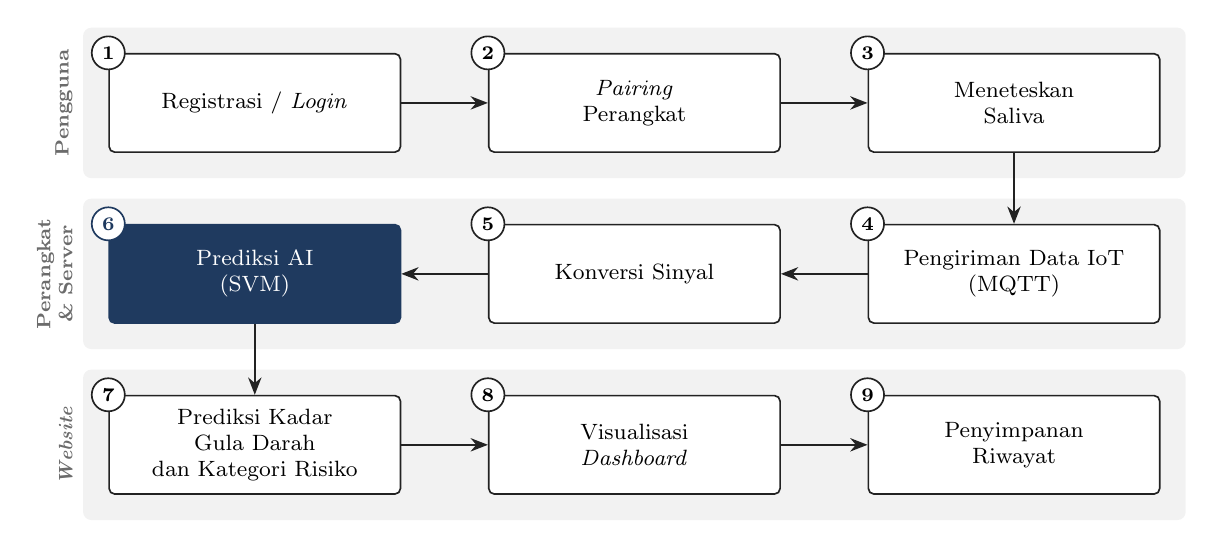
\begin{tikzpicture}[
  font=\footnotesize,
  >={Stealth[length=2.2mm,width=1.7mm]},
  line width=0.6pt,
  node distance=0.9cm and 1.1cm,
  tahap/.style={draw=ink, fill=white, rounded corners=2pt,
               minimum width=3.7cm, minimum height=1.25cm, text width=3.4cm,
               align=center, inner sep=3pt},
  ai/.style={tahap, draw=accent, fill=accent, text=white},
  num/.style={circle, draw=ink, fill=white, inner sep=0pt, minimum size=4.2mm,
              font=\scriptsize\bfseries},
  numai/.style={num, draw=accent, text=accent},
  flow/.style={->, draw=ink},
  lane/.style={fill=band, draw=none, rounded corners=3pt, inner sep=0.32cm},
  lanelbl/.style={font=\scriptsize\bfseries, text=mid, rotate=90, anchor=south, align=center},
]

% ---- Baris 1: Pengguna (kiri -> kanan) ----
\node[tahap]                 (s1) {Registrasi / \textit{Login}};
\node[tahap, right=of s1]    (s2) {\textit{Pairing}\\Perangkat};
\node[tahap, right=of s2]    (s3) {Meneteskan\\Saliva};

% ---- Baris 2: Perangkat & Server (kanan -> kiri) ----
\node[tahap, below=of s3]    (s4) {Pengiriman Data IoT\\(MQTT)};
\node[tahap, below=of s2]    (s5) {Konversi Sinyal};
\node[ai,   below=of s1]    (s6) {Prediksi AI\\(SVM)};

% ---- Baris 3: Hasil (kiri -> kanan) ----
\node[tahap, below=of s6]    (s7) {Prediksi Kadar Gula Darah\\dan Kategori Risiko};
\node[tahap, right=of s7]    (s8) {Visualisasi\\\textit{Dashboard}};
\node[tahap, right=of s8]    (s9) {Penyimpanan\\Riwayat};

% ---- Nomor tahap ----
\foreach \i in {1,...,9} {
  \ifnum\i=6
    \node[numai] at (s\i.north west) {\i};
  \else
    \node[num] at (s\i.north west) {\i};
  \fi
}

% ---- Panah alur (pola ular) ----
\draw[flow] (s1) -- (s2);
\draw[flow] (s2) -- (s3);
\draw[flow] (s3) -- (s4);
\draw[flow] (s4) -- (s5);
\draw[flow] (s5) -- (s6);
\draw[flow] (s6) -- (s7);
\draw[flow] (s7) -- (s8);
\draw[flow] (s8) -- (s9);

% ---- Lajur pelaku ----
\begin{scope}[on background layer]
  \node[lane, fit=(s1)(s3)] (L1) {};
  \node[lane, fit=(s6)(s4)] (L2) {};
  \node[lane, fit=(s7)(s9)] (L3) {};
\end{scope}
\node[lanelbl] at (L1.west) {Pengguna};
\node[lanelbl] at (L2.west) {Perangkat\\\& Server};
\node[lanelbl] at (L3.west) {\textit{Website}};

\end{tikzpicture}
\end{document}
